\section{Requirements \& Design}\label{sec:reqs}
%TODO elaborate on moscow; \cite{brennan2009}
Below we want to elaborate the requirements we put on this project and the design choices we made to meet them. To work out the initial set of requirements we followed the MoSCoW requirements scheme, yielding the following four priority-classes:
\begin{enumerate} \itemsep1pt \parskip0pt \parsep0pt
	\item{Must have}
		\begin{enumerate} \itemsep1pt \parskip0pt \parsep0pt
			\item{Individual Vehicle Simulation}
			\item{Vehicle Entrance \& Exit}
			\item{Diverse Vehicle Behaviours}
			\item{Statistics}
			\item{Traffic Management Policies}
		\end{enumerate}
	\item{Should have}
		\begin{enumerate} \itemsep1pt \parskip0pt \parsep0pt
			\item{Emergency Services}
			\item{User-defined Maps}
		\end{enumerate}
	\item{Could have}
		\begin{enumerate} \itemsep1pt \parskip0pt \parsep0pt
			\item{Import/Export of Maps and Settings}
			\item{External Map Source, e.g. Google Maps}
		\end{enumerate}
	\item{Won't have}
		\begin{enumerate} \itemsep1pt \parskip0pt \parsep0pt
			\item{Pre-exisiting Traffic Simulators or Third-Party Libraries}
		\end{enumerate}
\end{enumerate}

The delivered application is split in a map editor application and a simulator application. We will explain the design of and the requirements put on the simulator before introducing the map editing functionality in~\ref{ss-req-editor}.

\subsection{Simulator}
\subsubsection{Design}
%TODO tbc
* discrete time, continuous space
** tickrate, i.e. frequency of map updates
* all roads 4 lanes, 2 per dir, intersections with these and those paths, traffic lights, blocked-tiles
* overall approach: map contains square grid; map class does certain operations, mostly on behalf of the simulationcontroller. vehicles moving in continuous space but do occupy tiles as they move.

* first: discrete prototype, but problems, then continuous space model

* aimed for MVC but in the end turned out impractical, hence model and view 'verschmolzen', cf. cars being extension to rectangle class etc.

* Einheitenumrechnung Zeit, Speed, Beschleunigung\label{for:speedTransl}
\begin{equation}\label{for:speedTransl}	
\end{equation}


%this leads us to the first requirement...

\subsubsection{Requirements}
Requirement 1a, the simulation of individual vehicles, means that the simulation has to evaluate the behaviour of each car individually and draw conclusions for the traffic systems based on these observations. In simulation terms, we derive macroscopic statistics of a traffic network based on the aggregation of microscopic data.

\begin{wrapfigure}{t}{0.3\textwidth}
	\begin{center}
		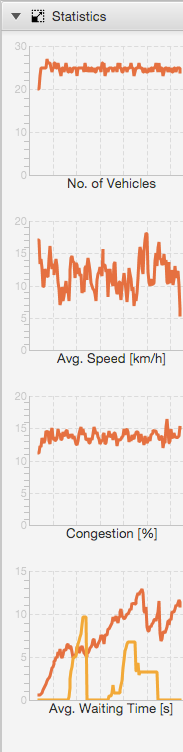
\includegraphics[scale=0.5]{img/graphs.png}
		\caption[Simulation Statistics at Runtime]{Simulation Statistics at Runtime}
		\label{fig:graphs}
	\end{center}
\end{wrapfigure}

During the simulation, vehicles enter the traffic network at one point, make their way through it, and exit it at an arbitrary touching-point of a road and the border of the map. (1b) On their way through the network, they exhibit different driving behaviours (1c), that is cautious drivers do not overtake and adjust their speed to surrounding cars while reckless drivers want to maximise their speed and overtake whenever possible.

The observations of the traffic network mentioned above are captured in live statistics at runtime of the simulation (1d).  We provide four charts measuring different network statistics. The first metric is the number of cars currently in the system, which gives a good reference point when analysing the trend of the other metrics. Secondly, we show the average speed of all present vehicles. The speed is given in km/h (cf. formula~\ref{for:speedTransl} for the unit conversion) and presented as arithmetic mean. That is, $ n^{-1}\sum\limits_{i=1}^n v_i$ for $n$ vehicles on the map and vehicle $i$ moving with velocity $v_i$. The third chart displayed shows the current congestion in the traffic network. Congestion is defined as the fraction of currently occupied tiles and the total number of tiles: $\frac{|\:\lbrace \:t\:|\:t\:\epsilon\:T\:\wedge\:t\:is\:occupied\rbrace\:|}{|\:T\:|}$, $T$ being the set of tiles. The last chart depicts two data series. First, the average time a normal vehicle had to wait on its way through the map and a second graph the average waiting time of an emergency vehicle. This chart illustrates nicely how the the fact that surrounding vehicles give way for emergency vehicles reduces their idle time in the traffic network. The displayed time is translated from simulation time into real time (i.e. multiplied by factor 10). The average is again shown as the arithmetic mean as follows: $10*n^{-1}\sum\limits_{i=1}^n w_i$, $w_i$ being the amount of simulation ticks vehicle $i$ has been idle. For improved readability, the statistics can be popped out of the user interface into a separate, resizable window (see button in top bar in Fig.~\ref{fig:graphs}). Additionally, the suite allows the export of the current simulation session's statistics into comma-separated-value format for further analysis.

When simulating the flow of cars in a traffic network it is of utmost importance to be able to alter the traffic management policies that are brought into effect (requirement 1e). Traffic management policies that are tangible in real-life situations include speed limits and the duration of red-light-phases of traffic lights. Besides these two, the Simulus simulation suite allows adjustment of the following simulation-specific policies: the maximum number of cars in the network, the tickrate of the simulation in milliseconds, the spawn delay, i.e. after how many ticks a new vehicle appears on the map, the ratio of cars to trucks (a value of 1 restricts trucks from spawning, 0 analogous), and lastly the ratio of reckless drivers to cautious drivers. All of the aforementioned but the traffic light duration are adjustable via sliders on the right side of the interface. Traffic light duration can be randomised for all traffic lights at once via a button, assigning a phase duration between 2000 and 5000 milliseconds.

The requirements discussed above comprised the \textit{Must have} category of our goals. The next requirement to mention is the implementation of emergency services (2a).
% emergency vehicles: ignore red lights, make other cars slow down and force them to give way
% always aim for max speed, double the acceleration of a normal car, 
% AoE


\subsection{Editor}\label{ss:req-editor}
